\chapter{传输层}

\section{多路复用与多路分解}

\subsection{传输层}

传输层协议为运行在不同主机上的应用进程之间提供了逻辑通信。在发送端,传输层将应用进程的报文添加传输层首部形成传输层分组,称为报文段(segment),这个过程被称为多路复用(multiplexing)。在接收端,网络层从数据报中提取传输层报文段,并交付给传输层,传输层处理报文段,将数据交付给应用进程,这个过程被称为多路分解(demultiplexing)。\\

应用层可以使用UDP和TCP这两种截然不同的传输层协议。其中UDP提供了一种不可靠、无连接的服务,因此,UDP不能保证一个进程发送的数据能够完整无缺地到达目的进程。而TCP提供了一种可靠的、面向连接的服务,通过使用流量控制、序号、确认和定时器,TCP确保正确地、按序地将数据交付给接收进程。\\

\subsection{无连接的多路复用/多路分解}

一个UDP的socket是由一个二元组进行标识的,该二元组包含了目的IP地址和目的端口号。如果两个UDP报文段来自不同的源IP地址或源端口号,但是具有相同的目的IP和目的端口号,那么这两个报文段将通过相同的socket被发送到相同的目的进程。\\

使用UDP时,当A给B发送的报文段中,源端口号是用作返回地址的一部分。当B回发一个报文段给A时,就需要从A到B的报文段中取值。\\

\begin{figure}[H]
	\centering
	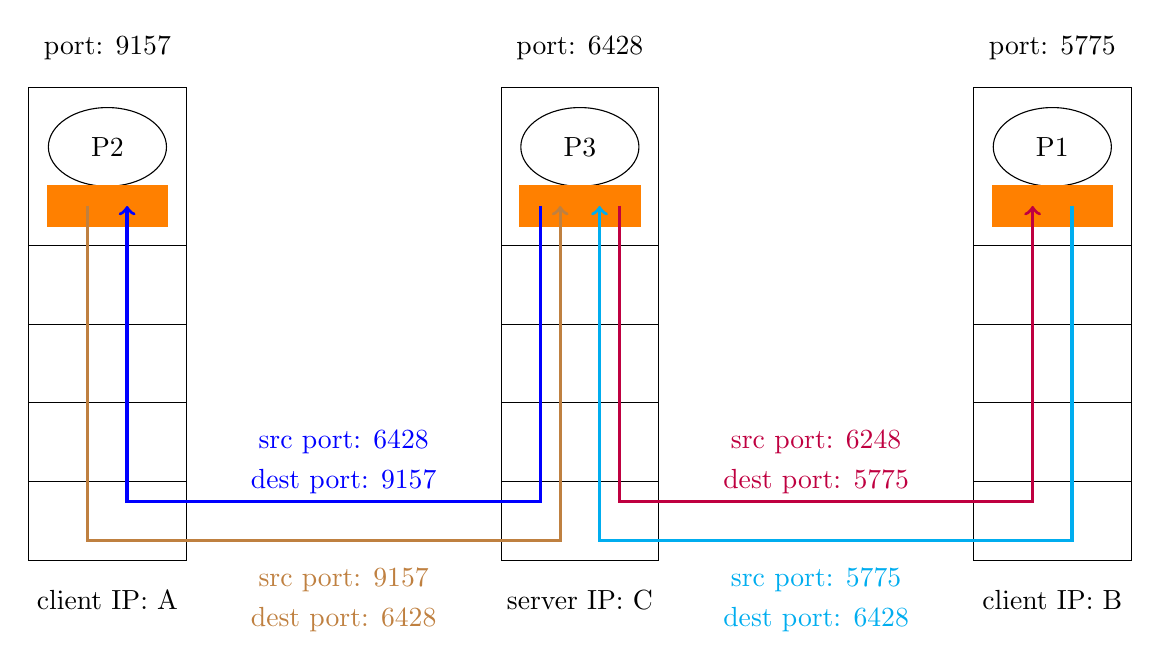
\begin{tikzpicture}
		\draw (1,6.5) node {port: 9157};
		\draw (0,0) rectangle (2,6);
		\draw (0,1) -- (2,1);
		\draw (0,2) -- (2,2);
		\draw (0,3) -- (2,3);
		\draw (0,4) -- (2,4);
		\draw (1,-0.5) node {client IP: A};
		\draw (1,5.25) ellipse (0.75 and 0.5);
		\draw (1,5.25) node {P2};
		\draw[orange, very thick, fill] (0.25,4.25) rectangle (1.75,4.75);

		\draw (7,6.5) node {port: 6428};
		\draw (6,0) rectangle (8,6);
		\draw (6,1) -- (8,1);
		\draw (6,2) -- (8,2);
		\draw (6,3) -- (8,3);
		\draw (6,4) -- (8,4);
		\draw (7,-0.5) node {server IP: C};
		\draw (7,5.25) ellipse (0.75 and 0.5);
		\draw (7,5.25) node {P3};
		\draw[orange, very thick, fill] (6.25,4.25) rectangle (7.75,4.75);

		\draw (13,6.5) node {port: 5775};
		\draw (12,0) rectangle (14,6);
		\draw (12,1) -- (14,1);
		\draw (12,2) -- (14,2);
		\draw (12,3) -- (14,3);
		\draw (12,4) -- (14,4);
		\draw (13,-0.5) node {client IP: B};
		\draw (13,5.25) ellipse (0.75 and 0.5);
		\draw (13,5.25) node {P1};
		\draw[orange, very thick, fill] (12.25,4.25) rectangle (13.75,4.75);

		\draw[->, very thick, brown] (0.75,4.5) -- (0.75,0.25) -- (6.75,0.25) -- (6.75,4.5);
		\draw[brown] (4,-0.25) node {src port: 9157};
		\draw[brown] (4,-0.75) node {dest port: 6428};

		\draw[->, very thick, blue] (6.5,4.5) -- (6.5,0.75) -- (1.25,0.75) -- (1.25,4.5);
		\draw[blue] (4,1.5) node {src port: 6428};
		\draw[blue] (4,1) node {dest port: 9157};

		\draw[->, very thick, cyan] (13.25,4.5) -- (13.25,0.25) -- (7.25,0.25) -- (7.25,4.5);
		\draw[cyan] (10,-0.25) node {src port: 5775};
		\draw[cyan] (10,-0.75) node {dest port: 6428};

		\draw[->, very thick, purple] (7.5,4.5) -- (7.5,0.75) -- (12.75,0.75) -- (12.75,4.5);
		\draw[purple] (10,1.5) node {src port: 6248};
		\draw[purple] (10,1) node {dest port: 5775};
	\end{tikzpicture}
	\caption{无连接的多路复用与多路分解}
\end{figure}

\vspace{0.5cm}

\subsection{面向连接的多路复用与多路分解}

TCP的socket是由一个四元组来标识的,其中包括了源IP地址、源端口号、目的IP地址和目的端口号。与UDP不同的是,两个具有不同源IP地址或源端口号的TCP报文段将被发送到两个不同的socket。\\

\begin{figure}[H]
	\centering
	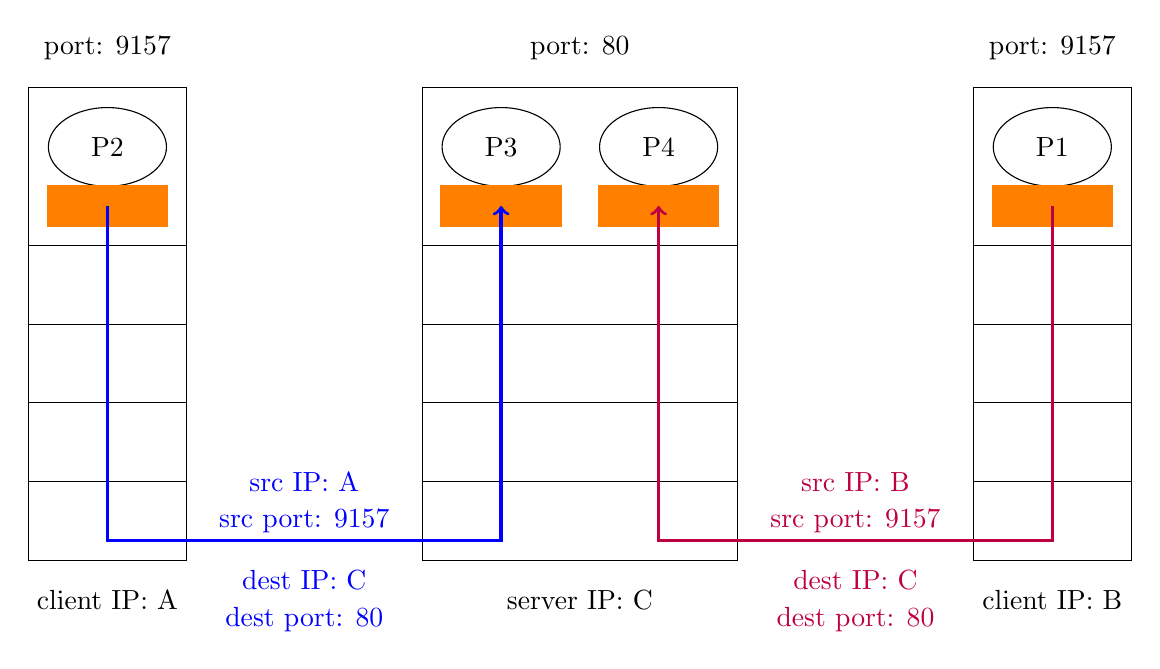
\begin{tikzpicture}
		\draw (1,6.5) node {port: 9157};
		\draw (0,0) rectangle (2,6);
		\draw (0,1) -- (2,1);
		\draw (0,2) -- (2,2);
		\draw (0,3) -- (2,3);
		\draw (0,4) -- (2,4);
		\draw (1,-0.5) node {client IP: A};
		\draw (1,5.25) ellipse (0.75 and 0.5);
		\draw (1,5.25) node {P2};
		\draw[orange, very thick, fill] (0.25,4.25) rectangle (1.75,4.75);

		\draw (7,6.5) node {port: 80};
		\draw (5,0) rectangle (9,6);
		\draw (5,1) -- (9,1);
		\draw (5,2) -- (9,2);
		\draw (5,3) -- (9,3);
		\draw (5,4) -- (9,4);
		\draw (7,-0.5) node {server IP: C};
		\draw (6,5.25) ellipse (0.75 and 0.5);
		\draw (6,5.25) node {P3};
		\draw[orange, very thick, fill] (5.25,4.25) rectangle (6.75,4.75);
		\draw (8,5.25) ellipse (0.75 and 0.5);
		\draw (8,5.25) node {P4};
		\draw[orange, very thick, fill] (7.25,4.25) rectangle (8.75,4.75);

		\draw (13,6.5) node {port: 9157};
		\draw (12,0) rectangle (14,6);
		\draw (12,1) -- (14,1);
		\draw (12,2) -- (14,2);
		\draw (12,3) -- (14,3);
		\draw (12,4) -- (14,4);
		\draw (13,-0.5) node {client IP: B};
		\draw (13,5.25) ellipse (0.75 and 0.5);
		\draw (13,5.25) node {P1};
		\draw[orange, very thick, fill] (12.25,4.25) rectangle (13.75,4.75);

		\draw[->, very thick, blue] (1,4.5) -- (1,0.25) -- (6,0.25) -- (6,4.5);
		\draw[blue] (3.5,1) node {src IP: A};
		\draw[blue] (3.5,0.5) node {src port: 9157};
		\draw[blue] (3.5,-0.25) node {dest IP: C};
		\draw[blue] (3.5,-0.75) node {dest port: 80};

		\draw[->, very thick, purple] (13,4.5) -- (13,0.25) -- (8,0.25) -- (8,4.5);
		\draw[purple] (10.5,1) node {src IP: B};
		\draw[purple] (10.5,0.5) node {src port: 9157};
		\draw[purple] (10.5,-0.25) node {dest IP: C};
		\draw[purple] (10.5,-0.75) node {dest port: 80};
	\end{tikzpicture}
	\caption{面向连接的多路复用与多路分解}
\end{figure}

\newpage

\section{无连接传输UDP}

\subsection{无连接传输UDP}

使用UDP时,在发送报文段之前,发送方和接收方的传输层实体之间没有握手。正因为如此,UDP被称为是无连接的。\\

UDP尽最大努力将数据包交付到目的主机,但不保证可靠性和顺序,也不保证带宽及延迟要求。UDP相较于TCP的优势包括无需连接建立、无连接状态、分组首部开销小。\\

\begin{table}[H]
	\centering
	\begin{tabular}{|p{3cm}<{\centering}|p{3cm}<{\centering}|}
		\hline
		source port \# & dest port \#                    \\
		\hline
		length         & checksum                        \\
		\hline
		\multicolumn{2}{|c|}{application data (message)} \\
		\hline
	\end{tabular}
	\caption{UDP报文段结构}
\end{table}

UDP首部只有4个字段,每个字段由2个字节组成,通过端口号可以将应用数据交给运行在目的端系统中的相应进程。长度字段指示了UDP报文段中的字节数(包括首部)。检验和可以用来检查该报文段中是否出现了差错。\\

\subsection{校验和(Checksum)}

当UDP报文段从源到达目的地的过程中,其中的bit有可能会受到噪声干扰或在路由器中存储而发生改变。UDP检验和提供了差错检测的功能。发送方对UDP报文段中所有内容都当作16位整数进行求和,在求和时遇到的溢出都需要被回卷(wraparound),再对和进行求反,得到的结果被放在UDP报文段中的检验和字段。\\

例如两个16位的整数相加:

\begin{table}[H]
	\centering
	\begin{tabular}{cD{.}{.}{3}}
		  & 1110011001100110  \\
		+ & 1101010101010101  \\
		\hline
		= & 11011101110111011
	\end{tabular}
\end{table}

将溢出位进行回卷:

\begin{table}[H]
	\centering
	\begin{tabular}{cD{.}{.}{3}}
		  & 1011101110111011 \\
		+ & 1                \\
		\hline
		= & 1011101110111100
	\end{tabular}
\end{table}

计算反码得到校验和0100010001000011。\\

接收方收到报文段后,将所有16位整数相加(包括检验和)。如果该分组中没有差错,则计算得到的和将是1111111111111111,否则说明分组中有差错。\\

当检验和错误的时候,该分组一定错误,将会被丢弃。但是当检验和没有错误时,并不能保证分组是完全正确的。虽然UDP提供差错检测,但它对差错恢复无能无力。

\newpage

\section{可靠数据传输}

\subsection{可靠数据传输(RDT, Reliable Data Transfer)}

由于可靠数据传输协议的下层协议也许是不可靠的,信道的不可靠特性决定了可靠数据传输协议的复杂性,例如TCP就是在不可靠的端到端网络层之上实现的可靠数据传输协议。\\

\begin{figure}[H]
	\centering
	\begin{tikzpicture}
		\draw (0,10) node {应用层};
		\draw (0,5) node {传输层};
		\draw (0,0) node {网络层};
		\draw[dashed] (0,7.5) -- (14,7.5);
		\draw[dashed] (0,2.5) -- (14,2.5);

		\draw (2,12) rectangle (3,13);
		\draw (5,12) rectangle (6,13);
		\draw (8,12) rectangle (9,13);
		\draw (11,12) rectangle (12,13);

		\draw (2.5,10) ellipse (0.75 and 0.5);
		\draw (2.5,10) node {发送};
		\draw (5.5,10) ellipse (0.75 and 0.5);
		\draw (5.5,10) node {接收};

		\node at (4.3,5) [cylinder, shape border rotate=180, draw, minimum height=2.5cm, minimum width=1cm]{可靠信道};
		\draw[->, very thick] (2.5,9.5) -- (2.5,5) -- (3,5);
		\draw[->, very thick] (5.4,5) -- (5.5,5) -- (5.5,9.5);

		\node at (10.3,0) [cylinder, shape border rotate=180, draw, minimum height=2.5cm, minimum width=1cm]{不可靠信道};
		\draw (7.5,4.5) rectangle (9.5,5.5);
		\draw (8.5,5) node {rdt};
		\draw (10.5,4.5) rectangle (12.5,5.5);
		\draw (11.5,5) node {rdt};

		\draw[->, very thick] (8.5,9) -- (8.5,5.5);
		\draw[->, very thick] (8.5,4.5) -- (8.5,0) -- (8.8,0);
		\draw[->, very thick] (11.5,0) -- (11.5,4.5);
		\draw[->, very thick] (11.5,5.5) -- (11.5,9);

		\draw (7,6.5) node {rdt\_send()};
		\draw (7,3.5) node {udt\_send()};
		\draw (13,6.5) node {deliver\_data()};
		\draw (13,3.5) node {udt\_rcv()};
	\end{tikzpicture}
	\caption{可靠数据传输}
\end{figure}

\vspace{0.5cm}

\subsection{rdt 1.0:经完全可靠信道的可靠数据传输}

考虑最简单的情况,假设底层信道是完全可靠的(不会出错、不会丢失)。有限状态机(FSM, Finite State Machine)可以用于描述发送方和接收方的操作。\\

\begin{figure}[H]
	\centering
	\begin{tikzpicture}
		\node[state, initial, draw, align=center] (s1) {wait for\\call};
		\draw (s1) edge[loop right] node{} (s1);
		\draw (5,0.5) node {rdt\_send(data)};
		\draw (2.5,0.25) -- (7.5,0.25);
		\draw (5,0) node {pkt = make\_pkt(data)};
		\draw (4.25,-0.5) node {udt\_send(pkt)};
	\end{tikzpicture}
	\caption{rdt 1.0发送端}
\end{figure}

\vspace{0.5cm}

\begin{figure}[H]
	\centering
	\begin{tikzpicture}
		\node[state, initial, draw, align=center] (s1) {wait for\\call};
		\draw (s1) edge[loop right] node{} (s1);
		\draw (5.5,0.5) node {rdt\_rcv(pkt)};
		\draw (3,0.25) -- (8,0.25);
		\draw (5.3,0) node {data = extract(pkt)};
		\draw (5.2,-0.5) node {deliver\_data(data)};
	\end{tikzpicture}
	\caption{rdt 1.0接收端}
\end{figure}

\vspace{0.5cm}

\subsection{rdt 2.0:经具有比特差错信道的可靠数据传输}

在分组的传输、传播或缓存的过程中,分组中的比特可能会受损。类似于打电话,当接听电话的人听到并理解一句话时会说“OK”,但如果没听清,就会要求对方再说一遍。\\

rdt 2.0增加了差错检验、接收方反馈和重传机制。当接收方接收到正确的报文时,就给对方一个肯定确认(ACK, positive acknowledgment),告诉他“没问题”。当接收方检测到报文错误时,就需要给对方一个否定确认(NAK, negative acknowledgment),告诉对方“你给我发的不对,重新给我发一份新的吧”。\\

\begin{figure}[H]
	\centering
	\begin{tikzpicture}[node distance=5cm]
		\node[state, initial, draw, align=center] (s1) {wait for\\call};
		\node[state, right of=s1, draw, align=center] (s2) {wait for\\ACK/NAK};

		\draw[->] (s1) edge[above, bend left] node{} (s2);
		\draw[->] (s2) edge[above, bend left] node{} (s1);
		\draw[->] (s2) edge[loop right] node{} (s2);

		\draw (0,3) node {rdt\_send(data)};
		\draw (-2.5,2.75) -- (2.5,2.75);
		\draw (0,2.5) node {sndpkt = make\_pkt(data)};
		\draw (-0.8,2) node {udt\_send(sndpkt)};

		\draw (9,2) node {rdt\_rcv(rcvpkt) \&\& is\_nak(rcvpkt)};
		\draw (5.5,1.75) -- (12.5,1.75);
		\draw (9,1.5) node {udt\_send(sndpkt)};

		\draw (3,-2) node {rdt\_rcv(rcvpkt) \&\& is\_ack(rcvpkt)};
		\draw (-0.5,-2.25) -- (6.5,-2.25);
		\draw (3,-2.5) node {$ \wedge $};
	\end{tikzpicture}
	\caption{rdt 2.0发送端}
\end{figure}

\vspace{0.5cm}

\begin{figure}[H]
	\centering
	\begin{tikzpicture}
		\node[state, initial, draw, align=center] (s1) {wait for\\call};
		\draw (s1) edge[loop above] node{} (s1);
		\draw (s1) edge[loop below] node{} (s1);

		\draw (4,3) node {rdt\_rcv(rcvpkt) \&\& corrupt(rcvpkt)};
		\draw (0.5,2.75) -- (7.5,2.75);
		\draw (3.5,2.5) node {sndpkt = make\_pkt(NAK)};
		\draw (2.65,2) node {udt\_send(sndpkt)};

		\draw (4,-1.5) node {rdt\_rcv(rcvpkt) \&\& !corrupt(rcvpkt)};
		\draw (0.5,-1.75) -- (7.5,-1.75);
		\draw (3.5,-2) node {data = extract(rcvpkt)};
		\draw (3.15,-2.5) node {deliver\_data(data)};
		\draw (3.95,-3) node {sndpkt = make\_pkt(ACK)};
		\draw (3.1,-3.5) node {udt\_send(sndpkt)};
	\end{tikzpicture}
	\caption{rdt 2.0接收端}
\end{figure}

\vspace{0.5cm}

发送方在将分组发送后,等待来自接收方的ACK或NAK。如果收到ACK,则代表接收方正确地接收了分组,那么就回到初始状态继续等待上层的数据。如果收到NAK,那就表示接收方没有收到正确的分组,需要进行重传并且继续处于等待ACK或NAK的状态。像这种只有当发送方接收到ACK后才能够继续发送新的报文的协议,被称为停等协议(stop-and-wait)。\\

rdt 2.0看起来似乎可以运行了,但遗憾的是,它存在一个致命的缺陷——ACK或NAK也存在受损的可能性!\\

当发送方收到的是一个受损的ACK或NAK时,如果发送方简单地选择直接重发分组会导致接收方收到重复的分组。\\

\subsection{rdt 2.1:带序号消息协议}

发送方可以为分组添加序号,接收方只需检查需要就可确定收到的分组是否重复。对于停等协议而言,序号只需要使用0和1就可以了。\\

\begin{figure}[H]
	\centering
	\begin{tikzpicture}[node distance=5cm]
		\node[state, initial, draw, align=center] (s1) {wait for\\call 0};
		\node[state, right of=s1, draw, align=center] (s2) {wait for\\ACK/NAK 0};
		\node[state, below of=s2, draw, align=center] (s3) {wait for\\call 1};
		\node[state, left of=s3, draw, align=center] (s4) {wait for\\ACK/NAK 1};

		\draw[->] (s1) edge[above, bend left] node{} (s2);
		\draw[->] (s2) edge[loop right] node{} (s2);
		\draw[->] (s2) edge[above, bend left] node{} (s3);
		\draw[->] (s3) edge[above, bend left] node{} (s4);
		\draw[->] (s4) edge[loop left] node{} (s4);
		\draw[->] (s4) edge[above, bend left] node{} (s1);

		\draw (3,3) node {rdt\_send(data)};
		\draw (0,2.75) -- (6,2.75);
		\draw (3,2.5) node {sndpkt = make\_pkt(0, data)};
		\draw (2,2) node {udt\_send(sndpkt)};

		\draw (8.5,2.5) node {rdt\_rcv(rcvpkt) \&\&};
		\draw (8.3,2) node {(corrupt(rcvpkt) ||};
		\draw (8.1,1.5) node {is\_nak(rcvpkt))};
		\draw (6.5,1.25) -- (10.5,1.25);
		\draw (8.5,1) node {udt\_send(sndpkt)};

		\draw (8,-2) node {rdt\_rcv(rcvpkt) \&\&};
		\draw (8,-2.5) node {!corrupt(rcvpkt) \&\&};
		\draw (7.6,-3) node {is\_ack(rcvpkt))};
		\draw (6,-3.25) -- (10,-3.25);
		\draw (7.5,-3.5) node {$ \wedge $};

		\draw (4,-7) node {rdt\_send(data)};
		\draw (1,-7.25) -- (7,-7.25);
		\draw (4,-7.5) node {sndpkt = make\_pkt(1, data)};
		\draw (3,-8) node {udt\_send(sndpkt)};

		\draw (-2,-7) node {rdt\_rcv(rcvpkt) \&\&};
		\draw (-2.2,-7.5) node {(corrupt(rcvpkt) ||};
		\draw (-2.4,-8) node {is\_nak(rcvpkt))};
		\draw (-4,-8.25) -- (0,-8.25);
		\draw (-2,-8.5) node {udt\_send(sndpkt)};

		\draw (-3,-2) node {rdt\_rcv(rcvpkt) \&\&};
		\draw (-3,-2.5) node {!corrupt(rcvpkt) \&\&};
		\draw (-3.4,-3) node {is\_ack(rcvpkt))};
		\draw (-5,-3.25) -- (-1,-3.25);
		\draw (-3,-3.5) node {$ \wedge $};
	\end{tikzpicture}
	\caption{rdt 2.1发送端}
\end{figure}

\vspace{0.5cm}

\begin{figure}[H]
	\centering
	\begin{tikzpicture}[node distance=5cm]
		\node[state, initial, draw, align=center] (s1) {wait for\\call 0};
		\node[state, right of=s1, draw, align=center] (s2) {wait for\\call 1};

		\draw[->] (s1) edge[above, bend left] node{} (s2);
		\draw[->] (s2) edge[above, bend left] node{} (s1);
		\draw[->] (s1) edge[loop above] node{} (s1);
		\draw[->] (s1) edge[loop below] node{} (s1);
		\draw[->] (s2) edge[loop above] node{} (s2);
		\draw[->] (s2) edge[loop below] node{} (s2);

		\draw (2.5,5) node {rdt\_rcv(rcvpkt) \&\&};
		\draw (2.5,4.5) node {!corrupt(rcvpkt) \&\&};
		\draw (2.2,4) node {has\_seq0(rcvpkt)};
		\draw (0.3,3.75) -- (5.7,3.75);
		\draw (2.6,3.5) node {data = extract(rcvpkt)};
		\draw (2.25,3) node {deliver\_data(data)};
		\draw (3,2.5) node {sndpkt = make\_pkt(ACK)};
		\draw (2.2,2) node {udt\_send(sndpkt)};

		\draw (-3.4,3) node {rdt\_rcv(rcvpkt) \&\&};
		\draw (-3.85,2.5) node {corrupt(rcvpkt)};
		\draw (-5.5,2.25) -- (-0.3,2.25);
		\draw (-2.75,2) node {sndpkt = make\_pkt(NAK)};
		\draw (-3.6,1.5) node {udt\_send(sndpkt)};

		\draw (-3.5,-2) node {rdt\_rcv(rcvpkt) \&\&};
		\draw (-3.5,-2.5) node {!corrupt(rcvpkt) \&\&};
		\draw (-3.7,-3) node {has\_seq1(rcvpkt)};
		\draw (-5.5,-3.25) -- (-0.3,-3.25);
		\draw (-2.8,-3.5) node {sndpkt = make\_pkt(ACK)};
		\draw (-3.65,-4) node {udt\_send(sndpkt)};

		\draw (2.5,-2) node {rdt\_rcv(rcvpkt) \&\&};
		\draw (2.5,-2.5) node {!corrupt(rcvpkt) \&\&};
		\draw (2.2,-3) node {has\_seq1(rcvpkt)};
		\draw (0.3,-3.25) -- (5.7,-3.25);
		\draw (2.6,-3.5) node {data = extract(rcvpkt)};
		\draw (2.25,-4) node {deliver\_data(data)};
		\draw (3,-4.5) node {sndpkt = make\_pkt(ACK)};
		\draw (2.2,-5) node {udt\_send(sndpkt)};

		\draw (7.7,3) node {rdt\_rcv(rcvpkt) \&\&};
		\draw (7.2,2.5) node {corrupt(rcvpkt)};
		\draw (5.5,2.25) -- (11,2.25);
		\draw (8.3,2) node {sndpkt = make\_pkt(NAK)};
		\draw (7.45,1.5) node {udt\_send(sndpkt)};

		\draw (8,-2) node {rdt\_rcv(rcvpkt) \&\&};
		\draw (8,-2.5) node {!corrupt(rcvpkt) \&\&};
		\draw (7.75,-3) node {has\_seq0(rcvpkt)};
		\draw (6,-3.25) -- (11.25,-3.25);
		\draw (8.65,-3.5) node {sndpkt = make\_pkt(ACK)};
		\draw (7.8,-4) node {udt\_send(sndpkt)};
	\end{tikzpicture}
	\caption{rdt 2.1接收端}
\end{figure}

\vspace{0.5cm}

\subsection{rdt 2.2:无NAK消息协议}

rdt 2.2与同rdt 2.1的功能相同,但是只使用ACK。接收方每次ACK最后一个被正确接收的分组,当发送方收到重复的ACK之后,采用与NAK相同的处理动作,将分组重传给接收方。\\

\begin{figure}[H]
	\centering
	\begin{tikzpicture}[node distance=4cm]
		\node[state, initial, draw, align=center] (s1) {wait for\\call 0};
		\node[state, right of=s1, draw, align=center] (s2) {wait for\\ACK 0};
		\node[state, below of=s2, draw, align=center] (s3) {wait for\\call 1};
		\node[state, left of=s3, draw, align=center] (s4) {wait for\\ACK 1};

		\draw[->] (s1) edge[above, bend left] node{} (s2);
		\draw[->] (s2) edge[loop right] node{} (s2);
		\draw[->] (s2) edge[above, bend left] node{} (s3);
		\draw[->] (s3) edge[above, bend left] node{} (s4);
		\draw[->] (s4) edge[loop left] node{} (s4);
		\draw[->] (s4) edge[above, bend left] node{} (s1);

		\draw (3,3) node {rdt\_send(data)};
		\draw (0,2.75) -- (6,2.75);
		\draw (3,2.5) node {sndpkt = make\_pkt(0, data)};
		\draw (2,2) node {udt\_send(sndpkt)};

		\draw (8.5,2.5) node {rdt\_rcv(rcvpkt) \&\&};
		\draw (8.3,2) node {(corrupt(rcvpkt) ||};
		\draw (8.3,1.5) node {is\_ack(rcvpkt, 1))};
		\draw (6.5,1.25) -- (10.5,1.25);
		\draw (8.5,1) node {udt\_send(sndpkt)};

		\draw (8,-1.5) node {rdt\_rcv(rcvpkt) \&\&};
		\draw (8,-2) node {!corrupt(rcvpkt) \&\&};
		\draw (7.9,-2.5) node {is\_ack(rcvpkt, 0))};
		\draw (6,-2.75) -- (10,-2.75);
		\draw (7.5,-3) node {$ \wedge $};

		\draw (4,-6) node {rdt\_send(data)};
		\draw (1,-6.25) -- (7,-6.25);
		\draw (4,-6.5) node {sndpkt = make\_pkt(1, data)};
		\draw (3,-7) node {udt\_send(sndpkt)};

		\draw (-2,-5.5) node {rdt\_rcv(rcvpkt) \&\&};
		\draw (-2.2,-6) node {(corrupt(rcvpkt) ||};
		\draw (-2.2,-6.5) node {is\_ack(rcvpkt, 0))};
		\draw (-4,-6.75) -- (0,-6.75);
		\draw (-2,-7) node {udt\_send(sndpkt)};

		\draw (-3,-1.5) node {rdt\_rcv(rcvpkt) \&\&};
		\draw (-3,-2) node {!corrupt(rcvpkt) \&\&};
		\draw (-3.2,-2.5) node {is\_ack(rcvpkt, 1))};
		\draw (-5,-2.75) -- (-1,-2.75);
		\draw (-3,-3) node {$ \wedge $};
	\end{tikzpicture}
	\caption{rdt 2.2发送端}
\end{figure}

\vspace{0.5cm}

\begin{figure}[H]
	\centering
	\begin{tikzpicture}[node distance=5cm]
		\draw[->] (-1,2) -- (-0.6,0.9);
		\draw (-1.5,1.5) node {start};

		\node[state, draw, align=center] (s1) {wait for\\call 0};
		\node[state, right of=s1, draw, align=center] (s2) {wait for\\call 1};

		\draw[->] (s1) edge[above, bend left] node{} (s2);
		\draw[->] (s2) edge[above, bend left] node{} (s1);
		\draw[->] (s1) edge[loop left] node{} (s1);
		\draw[->] (s2) edge[loop right] node{} (s2);

		\draw (1.8,5) node {rdt\_rcv(rcvpkt) \&\&};
		\draw (1.8,4.5) node {!corrupt(rcvpkt) \&\&};
		\draw (1.5,4) node {has\_seq0(rcvpkt)};
		\draw (-0.4,3.75) -- (5.5,3.75);
		\draw (1.9,3.5) node {data = extract(rcvpkt)};
		\draw (1.55,3) node {deliver\_data(data)};
		\draw (2.55,2.5) node {sndpkt = make\_pkt(ACK, 0)};
		\draw (1.5,2) node {udt\_send(sndpkt)};

		\draw (-3.5,-1) node {rdt\_rcv(rcvpkt) \&\&};
		\draw (-3.5,-1.5) node {(corrupt(rcvpkt) \&\&};
		\draw (-3.7,-2) node {has\_seq1(rcvpkt))};
		\draw (-5.5,-2.25) -- (0.5,-2.25);
		\draw (-2.65,-2.5) node {sndpkt = make\_pkt(ACK, 1)};
		\draw (-3.7,-3) node {udt\_send(sndpkt)};

		\draw (2.7,-1.5) node {rdt\_rcv(rcvpkt) \&\&};
		\draw (2.7,-2) node {!corrupt(rcvpkt) \&\&};
		\draw (2.4,-2.5) node {has\_seq1(rcvpkt)};
		\draw (0.5,-2.75) -- (5.9,-2.75);
		\draw (2.8,-3) node {data = extract(rcvpkt)};
		\draw (2.45,-3.5) node {deliver\_data(data)};
		\draw (3.4,-4) node {sndpkt = make\_pkt(ACK, 1)};
		\draw (2.4,-4.5) node {udt\_send(sndpkt)};

		\draw (7.7,3.5) node {rdt\_rcv(rcvpkt) \&\&};
		\draw (7.5,3) node {(corrupt(rcvpkt) ||};
		\draw (7.5,2.5) node {has\_seq0(rcvpkt))};
		\draw (5.5,2.25) -- (11.5,2.25);
		\draw (8.5,2) node {sndpkt = make\_pkt(ACK, 0)};
		\draw (7.45,1.5) node {udt\_send(sndpkt)};
	\end{tikzpicture}
	\caption{rdt 2.2接收端}
\end{figure}

\vspace{0.5cm}

\subsection{rdt 3.0:经具有比特差错的丢包信道的可靠数据传输}

假设现在信道既可能发生错误,也可能会丢失分组。如果发送端发送的数据在半路就丢失了,那么发送方就会无休止的等待,接收方没有收到数据,也会处于等待的状态。\\

因此发送方需要一个倒计时定时器(countdown timer),如果发送方在规定时间内没有收到ACK,就将该分组重传。另一种情况是,如果发送的分组并没有丢失,只是延误到达了,这样也会触发定时器重发。但是接收方可以根据分组的序号丢弃重复的分组。\\

\begin{figure}[H]
	\centering
	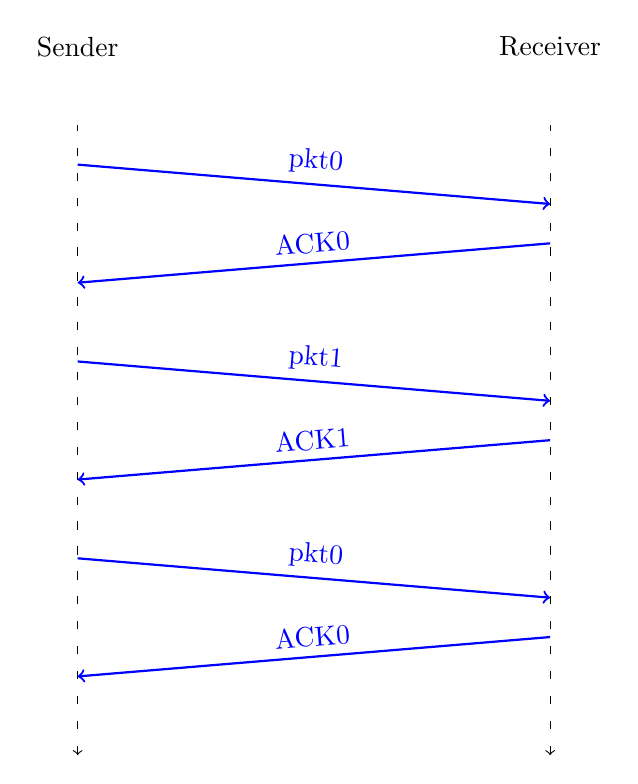
\begin{tikzpicture}
		\node at (0,9) {Sender};
		\node at (6,9) {Receiver};

		\draw[loosely dashed, <-] (0,0) -- (0,8);
		\draw[loosely dashed, <-] (6,0) -- (6,8);

		\draw[blue, ->, thick] (0,7.5) -- (6,7) node[above, midway, sloped]{pkt0};
		\draw[blue, ->, thick] (6,6.5) -- (0,6) node[above, midway, sloped]{ACK0};
		\draw[blue, ->, thick] (0,5) -- (6,4.5) node[above, midway, sloped]{pkt1};
		\draw[blue, ->, thick] (6,4) -- (0,3.5) node[above, midway, sloped]{ACK1};
		\draw[blue, ->, thick] (0,2.5) -- (6,2) node[above, midway, sloped]{pkt0};
		\draw[blue, ->, thick] (6,1.5) -- (0,1) node[above, midway, sloped]{ACK0};
	\end{tikzpicture}
	\caption{无丢包}
\end{figure}

\vspace{0.5cm}

\begin{figure}[H]
	\centering
	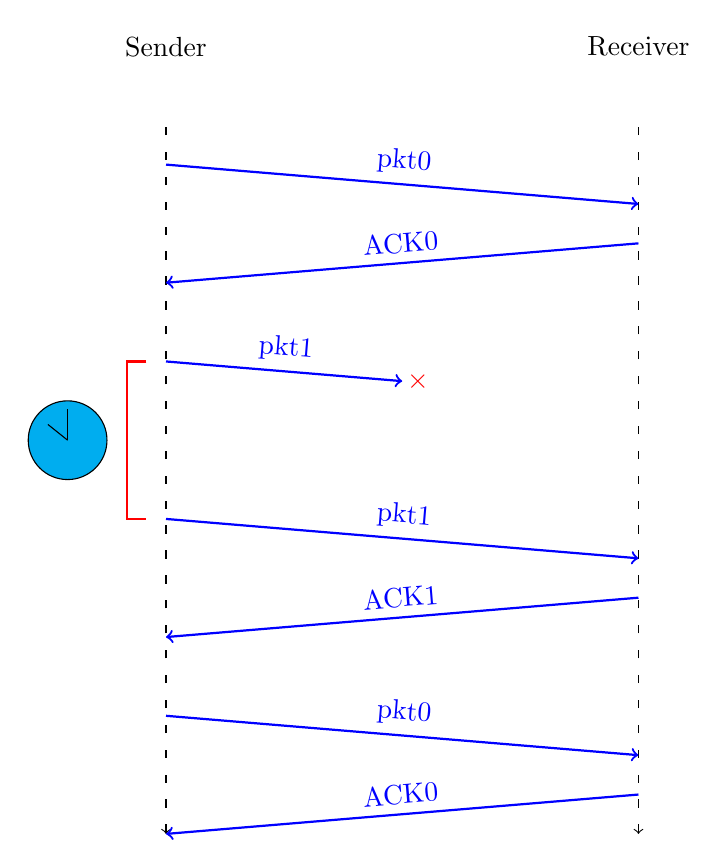
\begin{tikzpicture}
		\node at (0,10) {Sender};
		\node at (6,10) {Receiver};

		\draw[loosely dashed, <-] (0,0) -- (0,9);
		\draw[loosely dashed, <-] (6,0) -- (6,9);

		\draw[blue, ->, thick] (0,8.5) -- (6,8) node[above, midway, sloped]{pkt0};
		\draw[blue, ->, thick] (6,7.5) -- (0,7) node[above, midway, sloped]{ACK0};
		\draw[blue, ->, thick] (0,6) -- (3,5.75) node[above, midway, sloped]{pkt1};
		\node[very thick, red] at (3.2,5.75) {$ \times $};
		\draw[blue, ->, thick] (0,4) -- (6,3.5) node[above, midway, sloped]{pkt1};
		\draw[blue, ->, thick] (6,3) -- (0,2.5) node[above, midway, sloped]{ACK1};
		\draw[blue, ->, thick] (0,1.5) -- (6,1) node[above, midway, sloped]{pkt0};
		\draw[blue, ->, thick] (6,0.5) -- (0,0) node[above, midway, sloped]{ACK0};

		\draw[red, thick] (-0.25,6) -- (-0.5,6) -- (-0.5,4) -- (-0.25,4);
		\filldraw [fill=cyan] (-1.25,5) circle [radius=0.5cm];
		\draw (-1.25,5) -- (-1.25,5.4);
		\draw (-1.25,5) -- (-1.5,5.2);
	\end{tikzpicture}
	\caption{分组丢失}
\end{figure}

\vspace{0.5cm}

\begin{figure}[H]
	\centering
	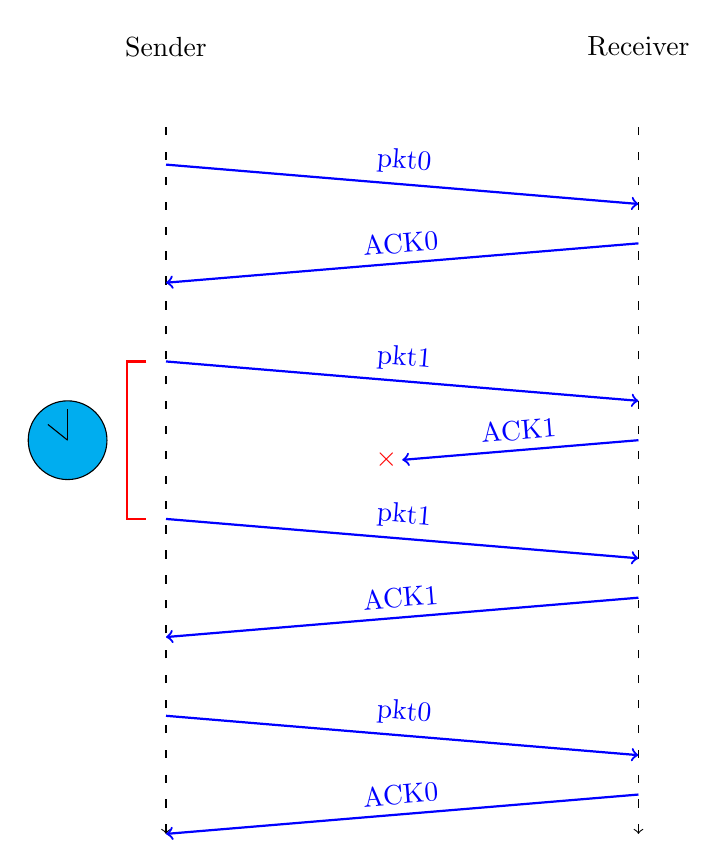
\begin{tikzpicture}
		\node at (0,10) {Sender};
		\node at (6,10) {Receiver};

		\draw[loosely dashed, <-] (0,0) -- (0,9);
		\draw[loosely dashed, <-] (6,0) -- (6,9);

		\draw[blue, ->, thick] (0,8.5) -- (6,8) node[above, midway, sloped]{pkt0};
		\draw[blue, ->, thick] (6,7.5) -- (0,7) node[above, midway, sloped]{ACK0};
		\draw[blue, ->, thick] (0,6) -- (6,5.5) node[above, midway, sloped]{pkt1};
		\draw[blue, ->, thick] (6,5) -- (3,4.75) node[above, midway, sloped]{ACK1};
		\node[very thick, red] at (2.8,4.75) {$ \times $};
		\draw[blue, ->, thick] (0,4) -- (6,3.5) node[above, midway, sloped]{pkt1};
		\draw[blue, ->, thick] (6,3) -- (0,2.5) node[above, midway, sloped]{ACK1};
		\draw[blue, ->, thick] (0,1.5) -- (6,1) node[above, midway, sloped]{pkt0};
		\draw[blue, ->, thick] (6,0.5) -- (0,0) node[above, midway, sloped]{ACK0};

		\draw[red, thick] (-0.25,6) -- (-0.5,6) -- (-0.5,4) -- (-0.25,4);
		\filldraw [fill=cyan] (-1.25,5) circle [radius=0.5cm];
		\draw (-1.25,5) -- (-1.25,5.4);
		\draw (-1.25,5) -- (-1.5,5.2);
	\end{tikzpicture}
	\caption{ACK丢失}
\end{figure}

\vspace{0.5cm}

\begin{figure}[H]
	\centering
	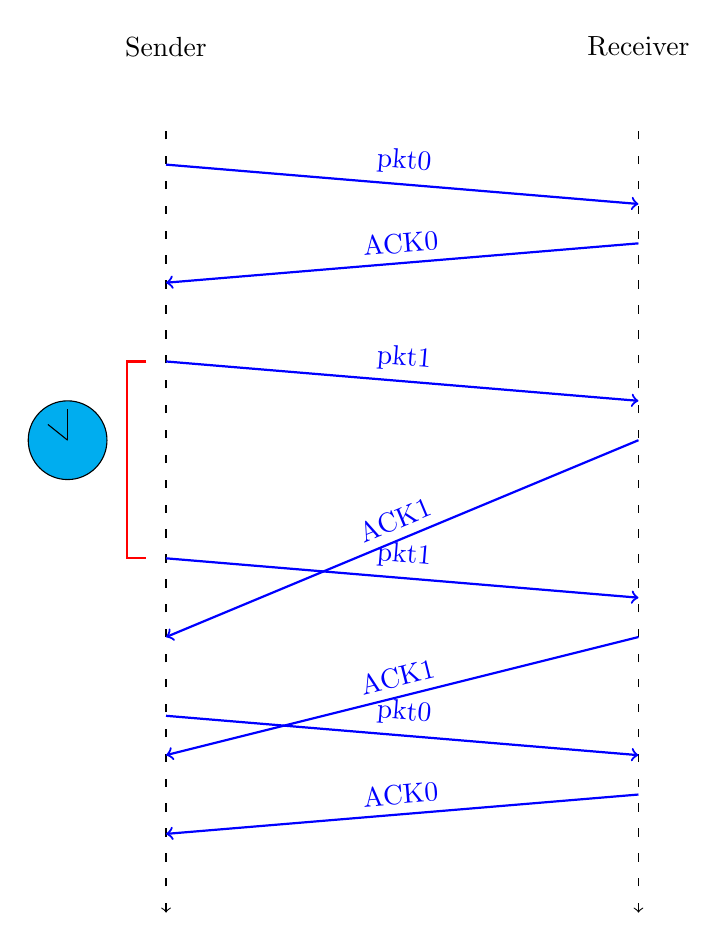
\begin{tikzpicture}
		\node at (0,11) {Sender};
		\node at (6,11) {Receiver};

		\draw[loosely dashed, <-] (0,0) -- (0,10);
		\draw[loosely dashed, <-] (6,0) -- (6,10);

		\draw[blue, ->, thick] (0,9.5) -- (6,9) node[above, midway, sloped]{pkt0};
		\draw[blue, ->, thick] (6,8.5) -- (0,8) node[above, midway, sloped]{ACK0};
		\draw[blue, ->, thick] (0,7) -- (6,6.5) node[above, midway, sloped]{pkt1};
		\draw[blue, ->, thick] (6,6) -- (0,3.5) node[above, midway, sloped]{ACK1};
		\draw[blue, ->, thick] (0,4.5) -- (6,4) node[above, midway, sloped]{pkt1};
		\draw[blue, ->, thick] (6,3.5) -- (0,2) node[above, midway, sloped]{ACK1};
		\draw[blue, ->, thick] (0,2.5) -- (6,2) node[above, midway, sloped]{pkt0};
		\draw[blue, ->, thick] (6,1.5) -- (0,1) node[above, midway, sloped]{ACK0};

		\draw[red, thick] (-0.25,7) -- (-0.5,7) -- (-0.5,4.5) -- (-0.25,4.5);
		\filldraw [fill=cyan] (-1.25,6) circle [radius=0.5cm];
		\draw (-1.25,6) -- (-1.25,6.4);
		\draw (-1.25,6) -- (-1.5,6.2);
	\end{tikzpicture}
	\caption{过早超时}
\end{figure}

\vspace{0.5cm}

rdt 3.0能够正确工作,但是性能很差。因为停等协议,导致了发送方的利用率很低。

\newpage

\section{流水线}

\subsection{流水线(Pipelining)}

为了提高发送方的利用率,可以不以停等方式运行,而是采用流水线协议,允许发送方在收到ACK之前连续发送多个分组。\\

使用流水线协议,就需要更大的序列号范围,因为每个输送中的分组必须有一个唯一的序号。同时发送方和接收方需要更大的存储空间以缓存分组。\\

\begin{figure}[H]
	\centering
	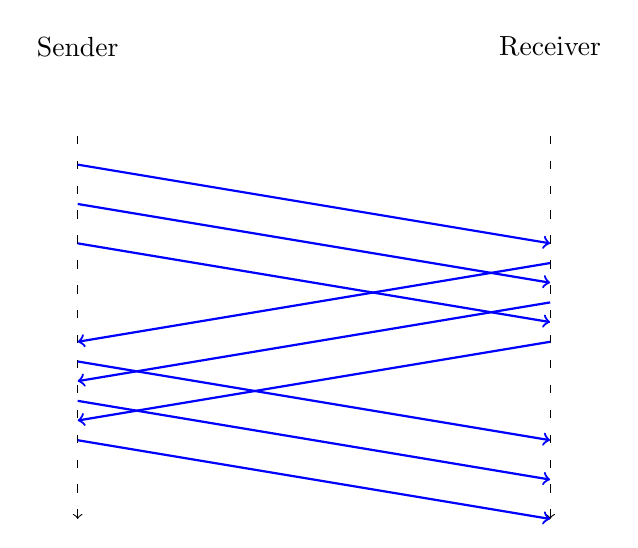
\begin{tikzpicture}
		\node at (0,6) {Sender};
		\node at (6,6) {Receiver};

		\draw[loosely dashed, <-] (0,0) -- (0,5);
		\draw[loosely dashed, <-] (6,0) -- (6,5);

		\draw[blue, ->, thick] (0,4.5) -- (6,3.5);
		\draw[blue, ->, thick] (0,4) -- (6,3);
		\draw[blue, ->, thick] (0,3.5) -- (6,2.5);
		\draw[blue, ->, thick] (6,3.25) -- (0,2.25);
		\draw[blue, ->, thick] (6,2.75) -- (0,1.75);
		\draw[blue, ->, thick] (6,2.25) -- (0,1.25);
		\draw[blue, ->, thick] (0,2) -- (6,1);
		\draw[blue, ->, thick] (0,1.5) -- (6,0.5);
		\draw[blue, ->, thick] (0,1) -- (6,0);
	\end{tikzpicture}
	\caption{流水线}
\end{figure}

解决流水线的差错恢复有两种基本方法:

\begin{enumerate}
	\item Go-Back-N
	\item 选择重传(Selective Repeat)
\end{enumerate}

\vspace{0.5cm}

\subsection{Go-Back-N (GBN)}

在GBN协议中,发送方允许发送多个分组,而不需等待确认。在GBN协议中,发送方的分组被分为4段。\\

\begin{figure}[H]
	\centering
	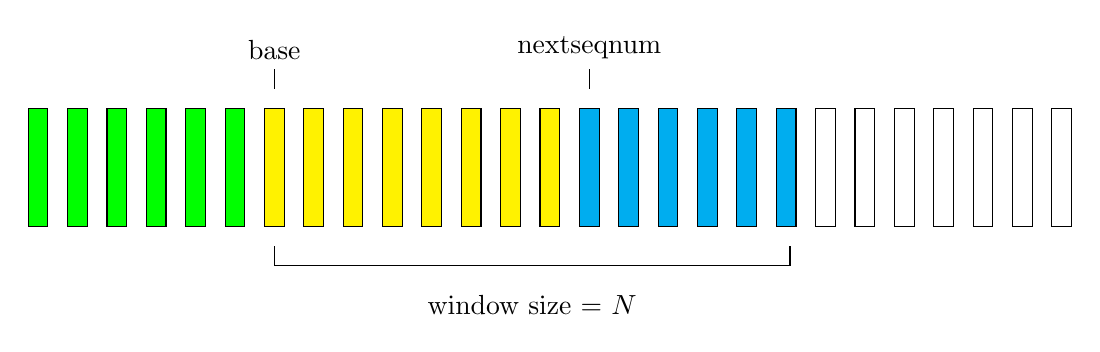
\begin{tikzpicture}
		\draw[fill=green] (0,0) rectangle (0.25,1.5);
		\draw[fill=green] (0.5,0) rectangle (0.75,1.5);
		\draw[fill=green] (1,0) rectangle (1.25,1.5);
		\draw[fill=green] (1.5,0) rectangle (1.75,1.5);
		\draw[fill=green] (2,0) rectangle (2.25,1.5);
		\draw[fill=green] (2.5,0) rectangle (2.75,1.5);

		\draw[fill=yellow] (3,0) rectangle (3.25,1.5);
		\draw[fill=yellow] (3.5,0) rectangle (3.75,1.5);
		\draw[fill=yellow] (4,0) rectangle (4.25,1.5);
		\draw[fill=yellow] (4.5,0) rectangle (4.75,1.5);
		\draw[fill=yellow] (5,0) rectangle (5.25,1.5);
		\draw[fill=yellow] (5.5,0) rectangle (5.75,1.5);
		\draw[fill=yellow] (6,0) rectangle (6.25,1.5);
		\draw[fill=yellow] (6.5,0) rectangle (6.75,1.5);

		\draw[fill=cyan] (7,0) rectangle (7.25,1.5);
		\draw[fill=cyan] (7.5,0) rectangle (7.75,1.5);
		\draw[fill=cyan] (8,0) rectangle (8.25,1.5);
		\draw[fill=cyan] (8.5,0) rectangle (8.75,1.5);
		\draw[fill=cyan] (9,0) rectangle (9.25,1.5);
		\draw[fill=cyan] (9.5,0) rectangle (9.75,1.5);

		\draw (10,0) rectangle (10.25,1.5);
		\draw (10.5,0) rectangle (10.75,1.5);
		\draw (11,0) rectangle (11.25,1.5);
		\draw (11.5,0) rectangle (11.75,1.5);
		\draw (12,0) rectangle (12.25,1.5);
		\draw (12.5,0) rectangle (12.75,1.5);
		\draw (13,0) rectangle (13.25,1.5);

		\draw (3.125,1.75) -- (3.125,2) node[above] {base};
		\draw (7.125,1.75) -- (7.125,2) node[above] {nextseqnum};
		\draw (3.125,-0.25) -- (3.125,-0.5) -- (9.675,-0.5) -- (9.675,-0.25);
		\node at (6.4,-1) {window size = $ N $};
	\end{tikzpicture}
	\caption{GBN滑动窗口}
\end{figure}

其中,$ [0, base - 1] $范围内的序号表示已经发送并被确认的分组,$ [base, nextseqnum - 1] $范围内的序号表示已经发送但未被确认的分组,$ [nextseqnum, base + N - 1] $范围内的序号表示等待被发送的分组,最后,大于等于$ base + N $的序号是不可用的。\\

随着协议的运行,窗口会在序号空间向前滑动,因此,GBN协议也常被称为滑动窗口协议(sliding-window protocol)。对于接收方,它的接收窗口为1,因此接收方将会丢弃所有失序的分组。\\

\begin{figure}[H]
	\centering
	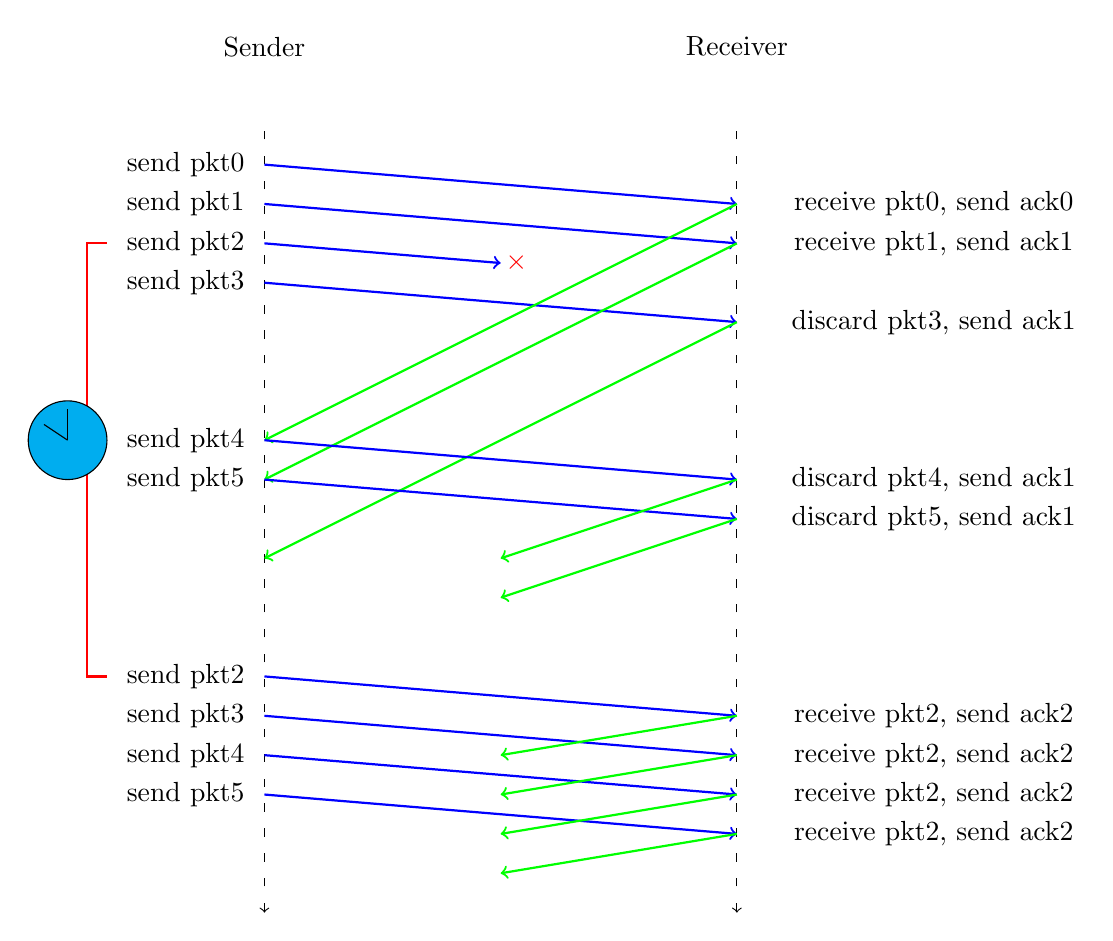
\begin{tikzpicture}
		\node at (0,11) {Sender};
		\node at (6,11) {Receiver};

		\draw[loosely dashed, <-] (0,0) -- (0,10);
		\draw[loosely dashed, <-] (6,0) -- (6,10);

		\draw[blue, ->, thick] (0,9.5) -- (6,9);
		\draw[blue, ->, thick] (0,9) -- (6,8.5);
		\draw[blue, ->, thick] (0,8.5) -- (3,8.25);
		\node[very thick, red] at (3.2,8.25) {$ \times $};
		\draw[blue, ->, thick] (0,8) -- (6,7.5);

		\draw[green, ->, thick] (6,9) -- (0,6);
		\draw[green, ->, thick] (6,8.5) -- (0,5.5);
		\draw[green, ->, thick] (6,7.5) -- (0,4.5);

		\draw[blue, ->, thick] (0,6) -- (6,5.5);
		\draw[blue, ->, thick] (0,5.5) -- (6,5);

		\draw[green, ->, thick] (6,5.5) -- (3,4.5);
		\draw[green, ->, thick] (6,5) -- (3,4);

		\draw[blue, ->, thick] (0,3) -- (6,2.5);
		\draw[blue, ->, thick] (0,2.5) -- (6,2);
		\draw[blue, ->, thick] (0,2) -- (6,1.5);
		\draw[blue, ->, thick] (0,1.5) -- (6,1);

		\draw[green, ->, thick] (6,2.5) -- (3,2);
		\draw[green, ->, thick] (6,2) -- (3,1.5);
		\draw[green, ->, thick] (6,1.5) -- (3,1);
		\draw[green, ->, thick] (6,1) -- (3,0.5);

		\node at (-1,9.5) {send pkt0};
		\node at (-1,9) {send pkt1};
		\node at (-1,8.5) {send pkt2};
		\node at (-1,8) {send pkt3};

		\node at (8.5,9) {receive pkt0, send ack0};
		\node at (8.5,8.5) {receive pkt1, send ack1};
		\node at (8.5,7.5) {discard pkt3, send ack1};

		\node at (-1,6) {send pkt4};
		\node at (-1,5.5) {send pkt5};

		\node at (8.5,5.5) {discard pkt4, send ack1};
		\node at (8.5,5) {discard pkt5, send ack1};

		\node at (-1,3) {send pkt2};
		\node at (-1,2.5) {send pkt3};
		\node at (-1,2) {send pkt4};
		\node at (-1,1.5) {send pkt5};

		\node at (8.5,2.5) {receive pkt2, send ack2};
		\node at (8.5,2) {receive pkt2, send ack2};
		\node at (8.5,1.5) {receive pkt2, send ack2};
		\node at (8.5,1) {receive pkt2, send ack2};

		\draw[red, thick] (-2,8.5) -- (-2.25,8.5) -- (-2.25,3) -- (-2,3);
		\filldraw [fill=cyan] (-2.5,6) circle [radius=0.5cm];
		\draw (-2.5,6) -- (-2.5,6.4);
		\draw (-2.5,6) -- (-2.8,6.2);
	\end{tikzpicture}
	\caption{GBN}
\end{figure}

\vspace{0.5cm}

\subsection{选择重传}

在GBN中,单个分组的差错就能够引起大量分组的重传,其中有很多分组其实是没有必要重传的。选择重传协议只需让发送方重传有差错的分组,而对于在窗口内已经接收的分组,将会把失序的分组缓存,直到重新接收到先前丢失的分组,这时才可以将这一批分组按序交付给上层。\\

\begin{figure}[H]
	\centering
	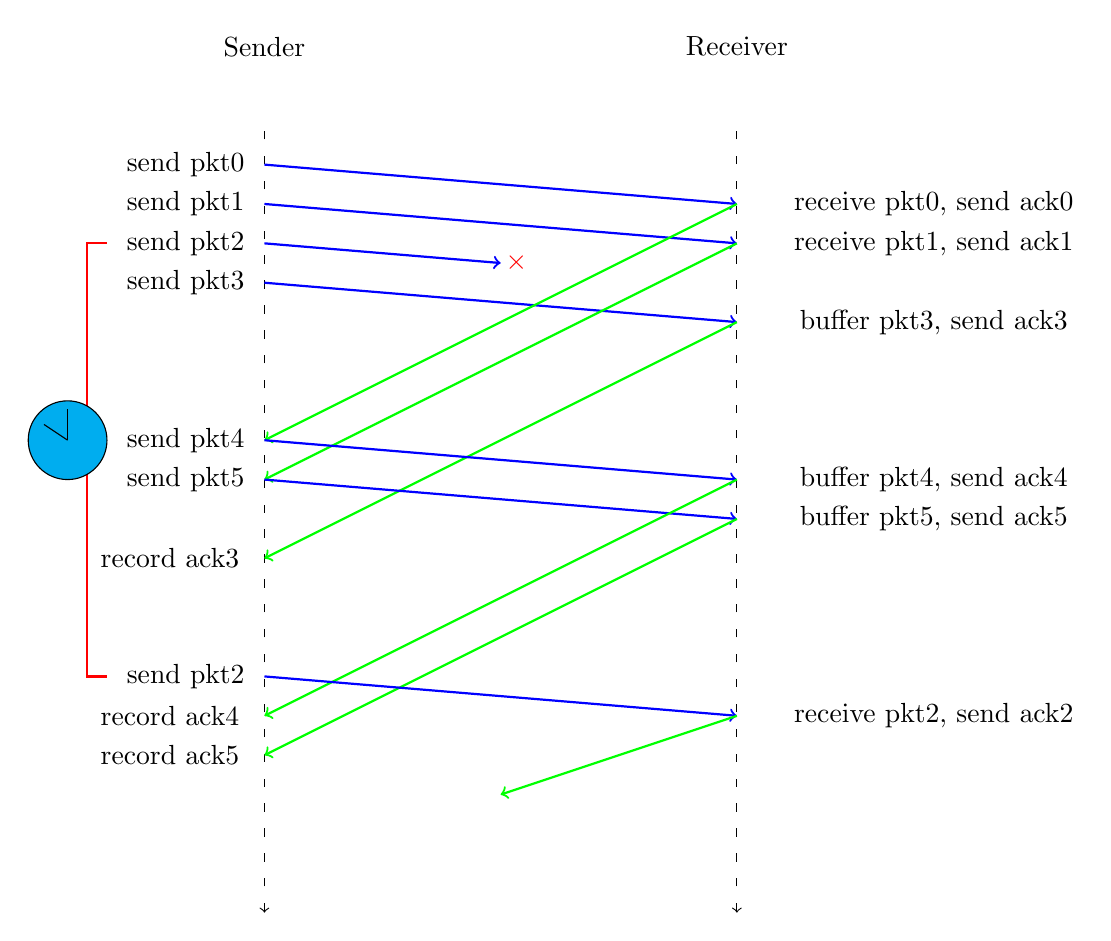
\begin{tikzpicture}
		\node at (0,11) {Sender};
		\node at (6,11) {Receiver};

		\draw[loosely dashed, <-] (0,0) -- (0,10);
		\draw[loosely dashed, <-] (6,0) -- (6,10);

		\draw[blue, ->, thick] (0,9.5) -- (6,9);
		\draw[blue, ->, thick] (0,9) -- (6,8.5);
		\draw[blue, ->, thick] (0,8.5) -- (3,8.25);
		\node[very thick, red] at (3.2,8.25) {$ \times $};
		\draw[blue, ->, thick] (0,8) -- (6,7.5);

		\draw[green, ->, thick] (6,9) -- (0,6);
		\draw[green, ->, thick] (6,8.5) -- (0,5.5);
		\draw[green, ->, thick] (6,7.5) -- (0,4.5);

		\draw[blue, ->, thick] (0,6) -- (6,5.5);
		\draw[blue, ->, thick] (0,5.5) -- (6,5);

		\draw[green, ->, thick] (6,5.5) -- (0,2.5);
		\draw[green, ->, thick] (6,5) -- (0,2);

		\draw[blue, ->, thick] (0,3) -- (6,2.5);

		\draw[green, ->, thick] (6,2.5) -- (3,1.5);

		\node at (-1,9.5) {send pkt0};
		\node at (-1,9) {send pkt1};
		\node at (-1,8.5) {send pkt2};
		\node at (-1,8) {send pkt3};

		\node at (8.5,9) {receive pkt0, send ack0};
		\node at (8.5,8.5) {receive pkt1, send ack1};
		\node at (8.5,7.5) {buffer pkt3, send ack3};

		\node at (-1,6) {send pkt4};
		\node at (-1,5.5) {send pkt5};

		\node at (8.5,5.5) {buffer pkt4, send ack4};
		\node at (8.5,5) {buffer pkt5, send ack5};

		\node at (-1.2,4.5) {record ack3};
		\node at (-1,3) {send pkt2};

		\node at (8.5,2.5) {receive pkt2, send ack2};

		\node at (-1.2,2.5) {record ack4};
		\node at (-1.2,2) {record ack5};

		\draw[red, thick] (-2,8.5) -- (-2.25,8.5) -- (-2.25,3) -- (-2,3);
		\filldraw [fill=cyan] (-2.5,6) circle [radius=0.5cm];
		\draw (-2.5,6) -- (-2.5,6.4);
		\draw (-2.5,6) -- (-2.8,6.2);
	\end{tikzpicture}
	\caption{选择重传}
\end{figure}

\newpage

\section{面向连接传输TCP}

\subsection{TCP报文段结构}

\begin{table}[!ht]
	\center
	\begin{tabular}{|c|c|c|c|c|c|c|c|c|c|c|}
		\hline
		\multicolumn{5}{|c|}{源端口号} & \multicolumn{6}{|c|}{目的端口号}                                              \\
		\hline
		\multicolumn{11}{|c|}{Sequence number}                                                                         \\
		\hline
		\multicolumn{11}{|c|}{Acknowledgment number}                                                                   \\
		\hline
		首部长度                       & Unused                             & C & E & U & A & P & R & S & F & 接收窗口 \\
		\hline
		\multicolumn{5}{|c|}{校验和}   & \multicolumn{6}{|c|}{紧急数据指针}                                            \\
		\hline
		\multicolumn{11}{|c|}{选项}                                                                                    \\
		\hline
		\multicolumn{11}{|c|}{数据}                                                                                    \\
		\hline
	\end{tabular}
	\caption{TCP报文段结构}
\end{table}

TCP报文段首部主要包括:

\begin{itemize}
	\item 源端口号/目的端口号:用于多路复用/分解上层应用的数据。

	\item 检验和:检测差错。

	\item 序号/确认号:用于实现可靠数据传输。

	\item 接收窗口:用于流量控制,指示接收方愿意接受的字节数。

	\item 首部长度:由于TCP选项字段,首部长度是可变的。通常选项字段为空,所以TCP首部的典型长度为20字节。

	\item ACK:指示确认字段中的值是有效的。

	\item RST/SYN/FIN:用于连接建立和拆除。
\end{itemize}

\vspace{0.5cm}

\subsection{序号与确认号}

TCP连接的双方都可以随机选择初始序号,这样可以降低上一条TCP连接残留的报文段被误认为是新连接的报文段的可能性(如果这两个连接恰好使用了同一个端口)。\\

主机A的确认号是主机A期望从主机B收到的下一字节的序号。因为TCP只确认该流中至第一个丢失字节为止的字节,所以TCP被称为提供累计确认。\\

Telnet是一个用于远程登录的应用层协议,它运行在TCP之上。假设主机A发起一个与主机B的Telnet会话,主机A的用于键入的每个字符都会被发送给主机B,主机B将回送每个字符的副本给主机A,并将这些字符显示在屏幕上,以确保发送的字符得到了处理。\\

假设主机A和B的初始序号为42和79,当用户输入一个字符后,这个字符会在网络中传输两次。\\

\begin{figure}[H]
	\centering
	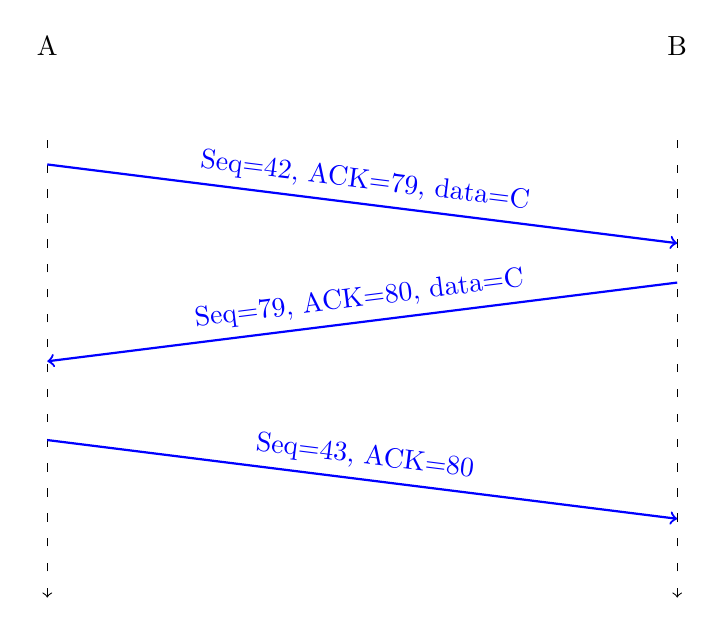
\begin{tikzpicture}
		\node at (0,7) {A};
		\node at (8,7) {B};

		\draw[loosely dashed, <-] (0,0) -- (0,6);
		\draw[loosely dashed, <-] (8,0) -- (8,6);

		\draw[blue, ->, thick] (0,5.5) -- (8,4.5) node[above, midway, sloped]{Seq=42, ACK=79, data=C};
		\draw[blue, ->, thick] (8,4) -- (0,3) node[above, midway, sloped]{Seq=79, ACK=80, data=C};
		\draw[blue, ->, thick] (0,2) -- (8,1) node[above, midway, sloped]{Seq=43, ACK=80};
	\end{tikzpicture}
	\caption{Telnet序号与确认号}
\end{figure}

\vspace{0.5cm}

\subsection{可靠数据传输}

TCP是建立在不可靠的、尽力而为的IP服务上的可靠数据传输协议,因此TCP采用了超时重传机制,确保了接收端收到的数据是有序无损的。\\

第一种情况是,假设主机A给主机B发送一个报文段,序号是92,包含8字节数据。在发出该报文段后,主机A需要等待来自主机B的确认号为100的报文段。虽然主机B收到了A的报文段,但是B发往A的确认报文丢失了。在这种情况下,超时事件就会发生。主机A会重传相同的报文段,当主机B收到重复报文将会将其丢弃。\\

\begin{figure}[H]
	\centering
	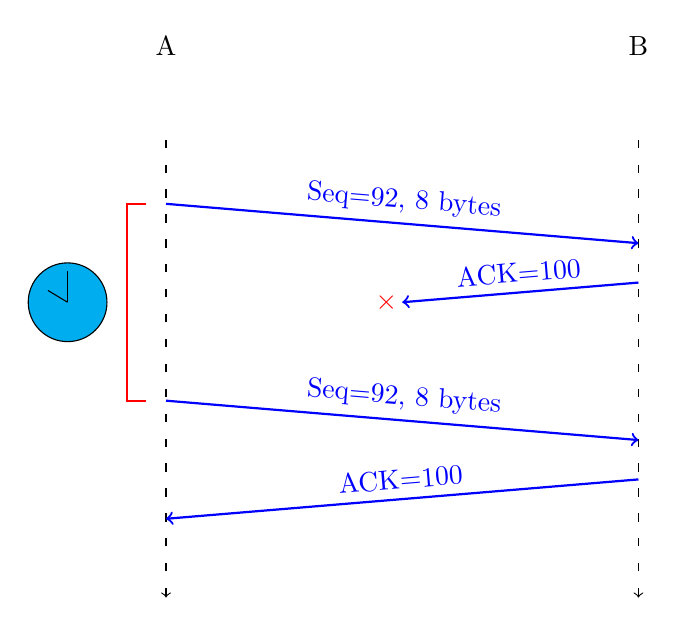
\begin{tikzpicture}
		\node at (0,7) {A};
		\node at (6,7) {B};

		\draw[loosely dashed, <-] (0,0) -- (0,6);
		\draw[loosely dashed, <-] (6,0) -- (6,6);

		\draw[blue, ->, thick] (0,5) -- (6,4.5) node[above, midway, sloped]{Seq=92, 8 bytes};
		\draw[blue, ->, thick] (6,4) -- (3,3.75) node[above, midway, sloped]{ACK=100};
		\node[very thick, red] at (2.8,3.75) {$ \times $};
		\draw[blue, ->, thick] (0,2.5) -- (6,2) node[above, midway, sloped]{Seq=92, 8 bytes};
		\draw[blue, ->, thick] (6,1.5) -- (0,1) node[above, midway, sloped]{ACK=100};

		\draw[red, thick] (-0.25,5) -- (-0.5,5) -- (-0.5,2.5) -- (-0.25,2.5);
		\filldraw [fill=cyan] (-1.25,3.75) circle [radius=0.5cm];
		\draw (-1.25,3.75) -- (-1.25,4.15);
		\draw (-1.25,3.75) -- (-1.5,3.9);
	\end{tikzpicture}
	\caption{确认丢失}
\end{figure}

\vspace{0.5cm}

第二种情况是,假设主机A连续发送了两个报文段,第一个报文段序号是92,包含8字节数据,第二个报文段序号是100,包含20字节数据。\\

这两个报文段都完好无损地到达主机B,并且主机B分别发送了确认号100和120,但是这两个确认报文都没有在超时之前到达。\\

当超时事件发生时,主机A将会重传序号为92的第一个报文段。此时,如果第二个报文段的ACK在新的超时之前到达,那么第二个报文段就不再会被重传。\\

\begin{figure}[H]
	\centering
	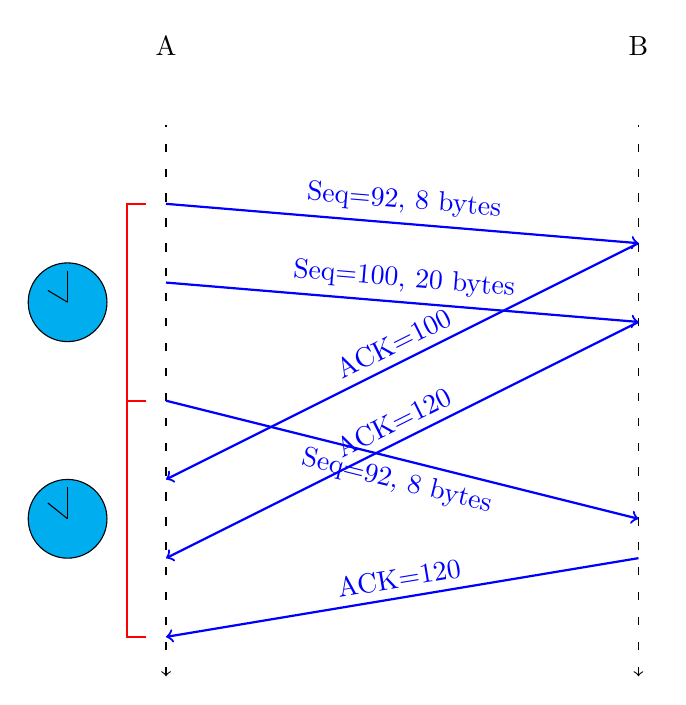
\begin{tikzpicture}
		\node at (0,8) {A};
		\node at (6,8) {B};

		\draw[loosely dashed, <-] (0,0) -- (0,7);
		\draw[loosely dashed, <-] (6,0) -- (6,7);

		\draw[blue, ->, thick] (0,6) -- (6,5.5) node[above, midway, sloped]{Seq=92, 8 bytes};
		\draw[blue, ->, thick] (0,5) -- (6,4.5) node[above, midway, sloped]{Seq=100, 20 bytes};
		\draw[blue, ->, thick] (6,5.5) -- (0,2.5) node[above, midway, sloped]{ACK=100};
		\draw[blue, ->, thick] (6,4.5) -- (0,1.5) node[above, midway, sloped]{ACK=120};
		\draw[blue, ->, thick] (0,3.5) -- (6,2) node[below, midway, sloped]{Seq=92, 8 bytes};
		\draw[blue, ->, thick] (6,1.5) -- (0,0.5) node[above, midway, sloped]{ACK=120};

		\draw[red, thick] (-0.25,6) -- (-0.5,6) -- (-0.5,3.5) -- (-0.25,3.5);
		\filldraw [fill=cyan] (-1.25,4.75) circle [radius=0.5cm];
		\draw (-1.25,4.75) -- (-1.25,5.15);
		\draw (-1.25,4.75) -- (-1.5,4.9);

		\draw[red, thick] (-0.25,3.5) -- (-0.5,3.5) -- (-0.5,0.5) -- (-0.25,0.5);
		\filldraw [fill=cyan] (-1.25,2) circle [radius=0.5cm];
		\draw (-1.25,2) -- (-1.25,2.4);
		\draw (-1.25,2) -- (-1.5,2.2);
	\end{tikzpicture}
	\caption{过早超时}
\end{figure}

\vspace{0.5cm}

第三种情况是,主机A发送两个报文段,其中第一个报文段的确认丢失,但是在超时事件发生之前,主机A收到了第二个报文段的确认。由于累计确认,主机知道主机B已经收到了之前所有的报文段,因此不会再重传。\\

\begin{figure}[H]
	\centering
	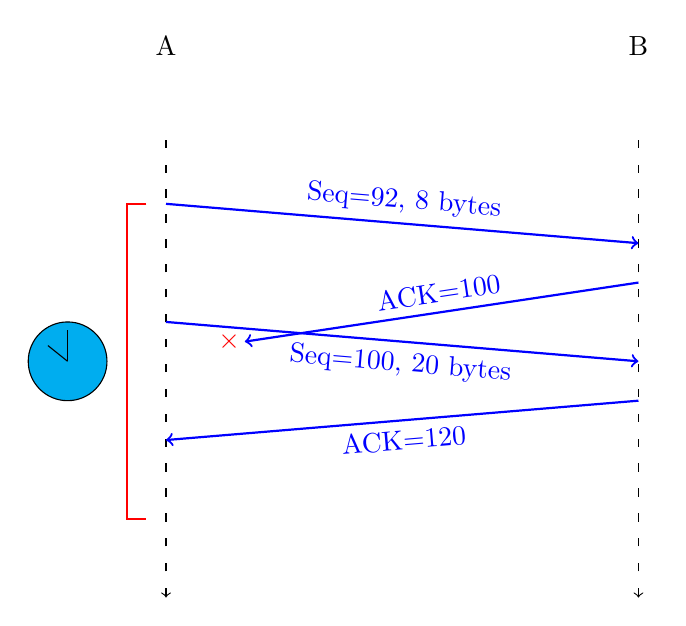
\begin{tikzpicture}
		\node at (0,7) {A};
		\node at (6,7) {B};

		\draw[loosely dashed, <-] (0,0) -- (0,6);
		\draw[loosely dashed, <-] (6,0) -- (6,6);

		\draw[blue, ->, thick] (0,5) -- (6,4.5) node[above, midway, sloped]{Seq=92, 8 bytes};
		\draw[blue, ->, thick] (6,4) -- (1,3.25) node[above, midway, sloped]{ACK=100};
		\node[very thick, red] at (0.8,3.25) {$ \times $};
		\draw[blue, ->, thick] (0,3.5) -- (6,3) node[below, midway, sloped]{Seq=100, 20 bytes};
		\draw[blue, ->, thick] (6,2.5) -- (0,2) node[below, midway, sloped]{ACK=120};

		\draw[red, thick] (-0.25,5) -- (-0.5,5) -- (-0.5,1) -- (-0.25,1);
		\filldraw [fill=cyan] (-1.25,3) circle [radius=0.5cm];
		\draw (-1.25,3) -- (-1.25,3.4);
		\draw (-1.25,3) -- (-1.5,3.2);
	\end{tikzpicture}
	\caption{累计确认}
\end{figure}

\vspace{0.5cm}

\subsection{快速重传(Fast Retransmit)}

超时触发重传存在一个问题,就是超时周期可能相对较长。当一个报文段丢失时,发送方就被迫延迟重传丢失的分组,因而增加了端到端时延。\\

通常,发送方可在超时事件发生之前,通过注意冗余的ACK可以检测到丢包情况。因为发送方发送大量的报文段,如果一个报文段丢失,就很可能引起许多冗余ACK。\\

如果发送方一旦收到3个冗余ACK,就认为该报文段已经丢失,TCP就会执行快速重传,即在该报文段超时之前就进行重传。\\

\begin{figure}[H]
	\centering
	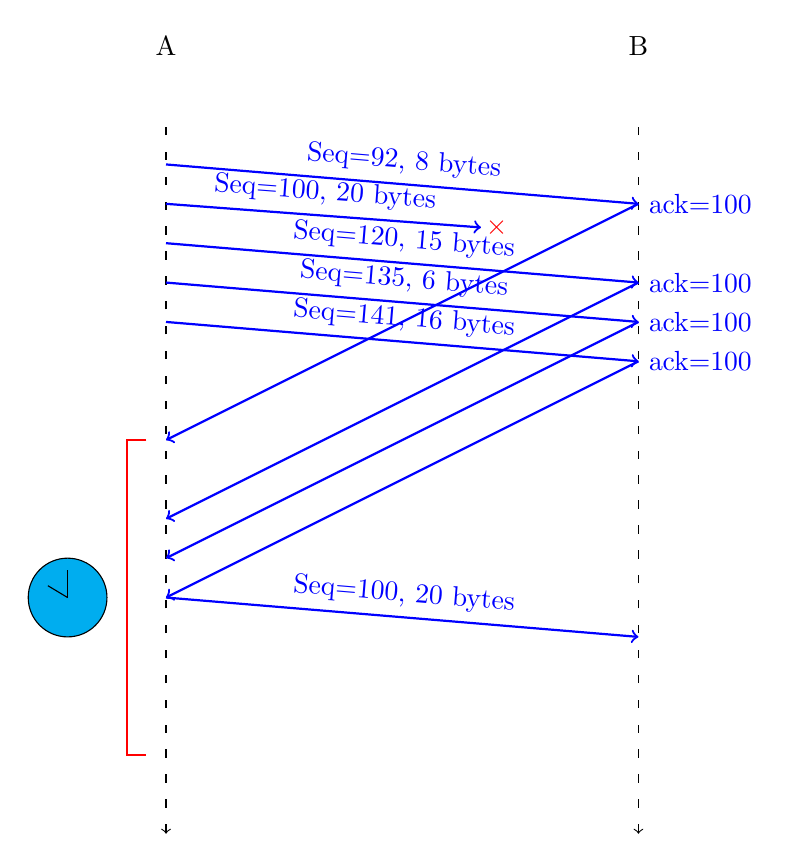
\begin{tikzpicture}
		\node at (0,10) {A};
		\node at (6,10) {B};

		\draw[loosely dashed, <-] (0,0) -- (0,9);
		\draw[loosely dashed, <-] (6,0) -- (6,9);

		\draw[blue, ->, thick] (0,8.5) -- (6,8) node[above, midway, sloped]{Seq=92, 8 bytes};
		\draw[blue, ->, thick] (0,8) -- (4,7.7) node[above, midway, sloped]{Seq=100, 20 bytes};
		\node[very thick, red] at (4.2,7.7) {$ \times $};
		\draw[blue, ->, thick] (0,7.5) -- (6,7) node[above, midway, sloped]{Seq=120, 15 bytes};
		\draw[blue, ->, thick] (0,7) -- (6,6.5) node[above, midway, sloped]{Seq=135, 6 bytes};
		\draw[blue, ->, thick] (0,6.5) -- (6,6) node[above, midway, sloped]{Seq=141, 16 bytes};

		\draw[blue, ->, thick] (6,8) node[right]{ack=100} -- (0,5);
		\draw[blue, ->, thick] (6,7) node[right]{ack=100} -- (0,4);
		\draw[blue, ->, thick] (6,6.5) node[right]{ack=100} -- (0,3.5);
		\draw[blue, ->, thick] (6,6) node[right]{ack=100} -- (0,3);

		\draw[blue, ->, thick] (0,3) -- (6,2.5) node[above, midway, sloped]{Seq=100, 20 bytes};

		\draw[red, thick] (-0.25,5) -- (-0.5,5) -- (-0.5,1) -- (-0.25,1);
		\filldraw [fill=cyan] (-1.25,3) circle [radius=0.5cm];
		\draw (-1.25,3) -- (-1.25,3.35);
		\draw (-1.25,3) -- (-1.5,3.15);
	\end{tikzpicture}
	\caption{快速重传}
\end{figure}

\vspace{0.5cm}

\subsection{TCP连接管理}

TCP的运输连接包括连接建立、数据传送和连接释放三个阶段。运输连接管理就是对连接建立以及连接释放过程的管控,使其能正常运行。\\

连接建立的过程被称为三次握手(three-way handshake):

\begin{enumerate}
	\item 第一次握手:客户端的应用进程主动打开,并向服务端发出请求报文段。其首部中,SYN=1、seq=x。
	
	\item 第二次握手:服务器应用进程被动打开,若同意客户端的请求,则发回确认报文。其首部中,SYN=1、ACK=1、ack=x+1、seq=y。

	\item 第三次握手:客户端收到确认报文后,通知上层应用进程连接已建立,并向服务器发出确认报文。其首部,ACK=1、ack=y+1。当服务器收到客户端的确认报文后,也通知其上层应用进程连接已建立。
\end{enumerate}

连接释放的过程被称为四次挥手:

\begin{enumerate}
	\item 第一次挥手:数据传输结束后,客户端应用进程发出连接释放报文段,并停止发送数据。其首部,FIN=1、seq=u。
	
	\item 第二次挥手:服务器收到连接释放报文段后,发出确认报文。其首部,ack=u+1、seq=v。此时本次连接就进入了半关闭状态,客户端不再向服务器发送数据,而服务器仍会继续发送。

	\item 第三次挥手:若服务器已经没有要向客户端发送的数据,其应用进程就通知服务器释放TCP连接。这个阶段服务器所发出的最后一个报文的首部中,FIN=1、ACK=1、seq=w、ack=u+1。
	
	\item 第四次挥手:客户端收到连接释放报文段后,必须发出确认,ACK=1、seq=u+1、ack=w+1。再经过2倍最长报文段寿命MSL(Maximum Segment Lifetime),本次TCP连接真正结束。
\end{enumerate}

\newpage